% =====================================================
%  Architecture & DDD — Full Slide Deck
% =====================================================
\documentclass[UTF8]{beamer}
\usetheme{Madrid}

% ----------- 套件 ----------
\usepackage{fontspec}
\usepackage{xcolor}
\usepackage{listings}
\usepackage{graphicx}
\usepackage{hyperref}
\hypersetup{colorlinks,linkcolor=black,urlcolor=blue}

\PassOptionsToPackage{quiet}{xeCJK}
\usepackage{ctex}
\setCJKmainfont{Noto Sans CJK TC}
\setCJKsansfont{Noto Sans CJK TC}
\setCJKmonofont{Noto Sans Mono CJK TC}

\usepackage{pgfpages}
\usepackage{tikz}
\usetikzlibrary{positioning}
\setbeameroption{show notes}

% ----------- 版面 ----------

\AtBeginSection[]{
  \begin{frame}
    \vfill
    \begin{center}
        \usebeamercolor{title}
        {\Huge \insertsection}
    \end{center}
    \vfill
  \end{frame}
}


% ----------- 程式碼顯示 ----------
\lstset{
  language=Java,
  basicstyle=\ttfamily\scriptsize,
  keywordstyle=\bfseries\color{blue},
  commentstyle=\itshape\color{gray},
  stringstyle=\color{purple},
  numbers=left, numberstyle=\tiny\color{gray}, numbersep=5pt,
  breaklines=true, showstringspaces=false,
  columns=flexible, tabsize=2,
  frame=single, framerule=0pt,
  backgroundcolor=\color{gray!6}
}

% ----------- 專案資訊 ----------
\title[第四章 · Architecture 與 DDD]{第四章:Architecture \\ 架構風格與 DDD 的協奏曲}
\date{}

% ======================================================
\begin{document}
% ------------------------------------------------------
\begin{frame}
    \titlepage
\end{frame}

% ------------------------------------------------------
\begin{frame}{目錄}
    \scriptsize
    \tableofcontents[hideallsubsections]
\end{frame}


% ================== Section: 引言 =====================
\section{開場}
\begin{frame}{開場引言}
    \begin{quote}
        \Large "Architecture should speak of its time and place,\\
        but yearn for timelessness."
        \small - \textit{Frank Gehry}
    \end{quote}
\end{frame}

\begin{frame}{核心觀點}
    \begin{itemize}
        \item DDD 是一套以 \textbf{Bounded Context} 劃界的思維框架,而非單一實作架構。
        \item 架構 = \textbf{品質屬性 + 功能需求} 的平衡藝術。
        \item 架構應服務於 Domain 模型;勿讓技術層凌駕業務語言。
        \item 追求可演進,抵禦未知需求,才能保持系統韌性。
    \end{itemize}
\end{frame}

% ================== Section: SaaSOvation =====================
\section{SaaSOvation 演進地圖}
\begin{frame}{SaaSOvation 架構演進}
    \scriptsize
    \begin{tabular}{|c|c|c|c|c|}
        \hline
        階段       & 架構               & 驅動     & 收穫       & 風險     \\ \hline\hline
        Startup    & Monolith (Layered) & MVP 速度 & 快速迭代   & 技術債   \\ \hline
        Scale-up   & Hexagonal + CQRS   & 可測試性 & 關注點分離 & 邊界模糊 \\ \hline
        Enterprise & 多 Context + SOA   & 團隊協作 & 去耦       & 協調成本 \\ \hline
    \end{tabular}
    \vspace{0.3cm}
    \begin{block}{啟示}
        沒有一步到位的架構:\bfseries{需求 × 風險 × 演進式重構} 才是真正的長青之道。
    \end{block}
\end{frame}

% ================== Section: Layered =====================
\section{Layered Architecture}
\begin{frame}{傳統分層架構 (Traditional Layers)}
    \begin{itemize}
        \item 傳統分層架構:UI → Application → Domain → Infrastructure
        \item 每層只能依賴自己和下層
        \item 優點:結構清晰、好上手
        \item 問題:Repository 介面在 Domain,實作在 Infrastructure
        \item 缺陷:違反層級規則、難以測試、技術層凌駕業務層
    \end{itemize}
    \begin{center}
        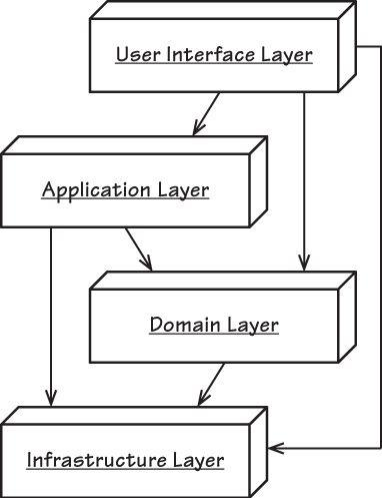
\includegraphics[width=0.3\textwidth]{img/layered-basic.png}
    \end{center}
\end{frame}

\begin{frame}{依賴反轉原則 (DIP)}
    \begin{itemize}
        \item 高階模組不應依賴低階模組,兩者都應依賴抽象
        \item 抽象不應依賴細節,細節應依賴抽象
        \item 解決方案:引入 DIP
        \item 邏輯上將 Infrastructure 層「移至上層」
        \item 實際上是讓 Infrastructure 實作 Domain 定義的介面
    \end{itemize}
\end{frame}
\begin{frame}[fragile]{Layered Java (DIP)}
    \tiny
    \begin{lstlisting}
@Transactional
public void commitBacklogItemToSprint(
    String aTenantId, String aBacklogItemId, String aSprintId) {
    TenantId tenantId = new TenantId(aTenantId);
    BacklogItem backlogItem =
        backlogItemRepository.backlogItemOfId(
            tenantId, new BacklogItemId(aBacklogItemId));
    Sprint sprint = sprintRepository.sprintOfId(
        tenantId, new SprintId(aSprintId));
    backlogItem.commitTo(sprint);
}
\end{lstlisting}
\end{frame}

\begin{frame}[fragile]{Layered Java (DIP)}
    \tiny
    \begin{lstlisting}
package
com.saasovation.agilepm.infrastructure.persistence;
import com.saasovation.agilepm.domain.model.product.*;
public class HibernateBacklogItemRepository
implements BacklogItemRepository {
...
@Override
@SuppressWarnings("unchecked")
public Collection<BacklogItem>
allBacklogItemsComittedTo(
Tenant aTenant, SprintId aSprintId) {
Query query =
this.session().createQuery(
"from -BacklogItem as _obj_ "
+ "where _obj_.tenant = ? and
_obj_.sprintId = ?");
query.setParameter(0, aTenant);
query.setParameter(1, aSprintId);
return (Collection<BacklogItem>) query.list();
}
...
}
\end{lstlisting}
\end{frame}

\begin{frame}{DIP:分層的變革}
    \begin{itemize}
        \item 傳統分層架構是「高階元件依賴低階元件」
        \item DIP 顛倒依賴方向:Domain 定義介面,Infrastructure 實作
        \item Infrastructure 被「邏輯上」放在最上層
        \item 它是「實作者」,不是「控制者」
        \item 符合 DDD 精神:Domain 是中心,技術在外圍服務它
    \end{itemize}
    \begin{center}
        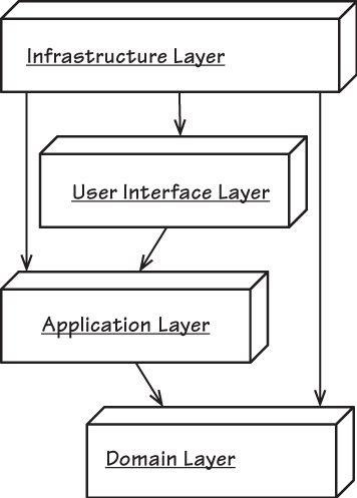
\includegraphics[width=0.3\textwidth]{img/infra-calls-domain.png}
    \end{center}
\end{frame}

% ================== Section: Hexagonal =====================
\section{Hexagonal Architecture}
\begin{frame}{Hexagonal 架構三大核心}
    \begin{enumerate}
        \item 所有依賴都「向內」指向應用核心(Domain + Use Cases)
        \item 對外協定由 Adapter 處理(如 HTTP、AMQP、JDBC)
        \item Application Service 對 Port 發出請求,由 Adapter 實作
    \end{enumerate}
    \vspace{0.5em}
    \textbf{→ 避免耦合框架,實現技術可替換性、測試友善性、邊界清晰性}
    \begin{center}
        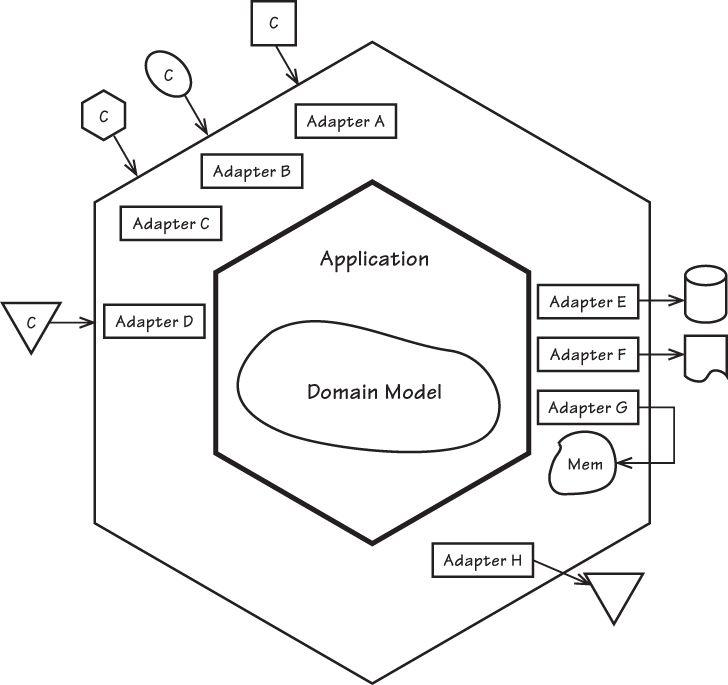
\includegraphics[width=0.5\textwidth]{img/hexagonal-architecture.png}
    \end{center}
\end{frame}

\begin{frame}[fragile]{Hexagonal 架構 Input Port Java 範例}
    \scriptsize
    \begin{lstlisting}[language=Java]
// === Input Adapter ===
@Path("/tenants/{tenantId}/products") // 接收 HTTP 請求,是 Input Adapter
public class ProductResource extends Resource {
    // === Port ===
    private ProductService productService; // 這是 Input Port(介面)
    @GET
    @Path("{productId}")
    @Produces({"application/vnd.saasovation.projectovation+xml"})
    public Product getProduct(
        @PathParam("tenantId") String aTenantId,
        @PathParam("productId") String aProductId,
        @Context Request aRequest) {
        // 呼叫 Port 的方法,將外部資料導入應用層(Port 實作中會使用 Domain Model)
        Product product = productService.product(aTenantId, aProductId);
        if (product == null) {
            throw new WebApplicationException(Response.Status.NOT_FOUND);
        }
        // 回傳的是 Domain 物件,由 Output Adapter(MessageBodyWriter)序列化為 XML
        return product;
    }
}
\end{lstlisting}
\end{frame}

\begin{frame}[shrink=20]{Hexagonal 架構的 Port 與 Adapter}
    \begin{center}
        \textit{依賴方向皆由外往內,所有 Adapter 實作 Port,所有 Port 為內部定義}
    \end{center}
    \begin{center}
        \begin{tikzpicture}[node distance=1.2cm, every node/.style={align=center}]
            % 上方輸入流
            \node (uiAdapter) [draw, rectangle] {ProductResource\\(Input Adapter)};
            \node (http) [below=of uiAdapter, draw, rectangle] {HTTP / JAX-RS\\(技術協定)};
            \node (port) [below=of http, draw, rectangle] {ProductService\\(Input Port)};
            \node (app) [below=of port, draw, rectangle] {ProductApplicationService\\(Use Case 實作)};

            % 下方輸出流
            \node (repoPort) [below=of app, draw, rectangle] {ProductRepository\\(Output Port)};
            \node (repoImpl) [below left=1cm and 0.5cm of repoPort, draw, rectangle] {MySQLRepository\\(Output Adapter)};
            \node (msgAdapter) [below right=1cm and 0.5cm of repoPort, draw, rectangle] {MessageBodyWriter\\(Output Adapter)};

            % arrows
            \draw[->] (uiAdapter) -- node[right] {轉接協定} (http);
            \draw[->] (http) -- node[right] {呼叫 Port} (port);
            \draw[->] (port) -- node[right] {由 Use Case 實作} (app);
            \draw[->] (app) -- node[right] {依賴} (repoPort);
            \draw[->] (repoImpl) -- node[left] {實作} (repoPort);
            \draw[->] (msgAdapter) -- node[right] {輸出格式} (repoPort);
        \end{tikzpicture}
    \end{center}
\end{frame}


\begin{frame}{Hexagonal 架構的 DDD 價值}
    \begin{itemize}
        \item 隔離技術細節,讓核心 Domain 不依賴外部框架
        \item 測試容易:可以在無 UI / 無 DB 下進行完整測試
        \item 高擴充性:新增一種協定只需新增對應 Adapter
        \item 是實踐 DDD 的最佳部署架構之一
    \end{itemize}
\end{frame}

% ================== Section: SOA =====================
\section{SOA Architecture}
\begin{frame}{SOA 架構精要}
    \begin{itemize}
        \item 每個 Bounded Context → 獨立服務 (Service)
        \item 技術介面可為 REST / SOAP / Messaging
        \item 不同技術服務可共享同一語意邊界(如一組 REST + Queue 為一 BC 的對外服務)
        \item 一個業務服務 = 多個技術服務 + 多個 Bounded Context
        \item 治理與韌性:Registry、Contract-First、Versioning、Circuit Breaker、Retry 等
    \end{itemize}
\end{frame}

\begin{frame}{Hexagonal Architecture supporting SOA, with REST, SOAP, and messaging services}
    \begin{center}
        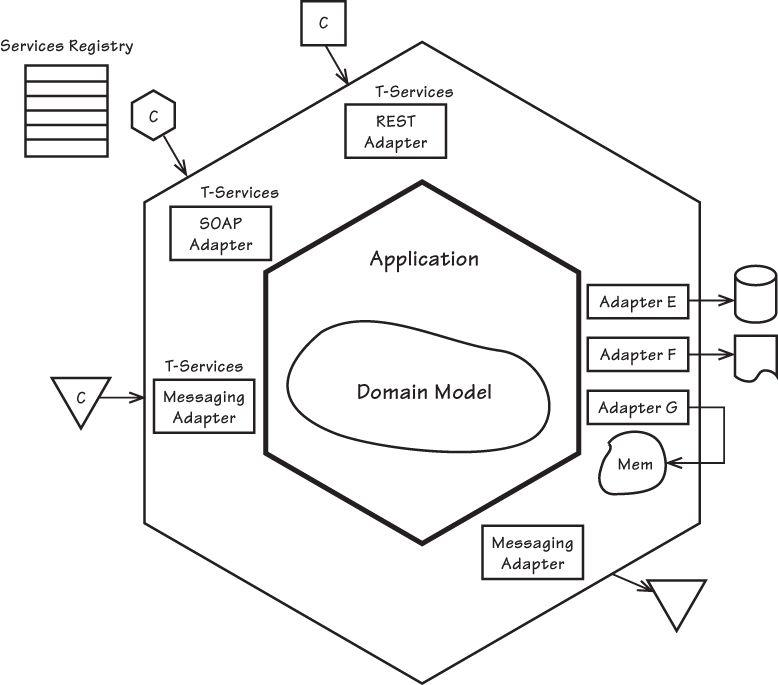
\includegraphics[width=0.7\textwidth]{img/hexagonal-tservice.png}
    \end{center}
\end{frame}


% ================== Section: REST =====================
\section{REST architectural style}

\begin{frame}{Contract-First Design}
    \begin{itemize}
        \item 先編寫明確的介面定義(「合約」),再實作服務程式碼
        \item 合約成為單一事實來源:
        \begin{itemize}
            \item \textbf{Provider}:依照合約生成或手寫服務端程式碼
            \item \textbf{Consumer}:生成存根/SDK 或用於驗證與模擬
            \item \textbf{Governance}:版本控制、相容性檢查、策略執行、文件
        \end{itemize}
    \end{itemize}
    \tiny
    \begin{center}
        \begin{tabular}{|l|l|l|}
            \hline
            \textbf{協定} & \textbf{合約格式} & \textbf{程式碼生成工具} \\
            \hline
            REST/HTTP & OpenAPI 3 / AsyncAPI & Swagger Codegen, openapi-generator \\
            \hline
            gRPC & Protocol Buffers (.proto) & protoc, Buf, Grpc-Tools \\
            \hline
            SOAP & WSDL + XSD & wsimport, wsdl2java \\
            \hline
            Events & Avro Schema, AsyncAPI & avro-tools, Karate, Springs Cloud Stream \\
            \hline
        \end{tabular}
    \end{center}
\end{frame}

\begin{frame}{為何選擇 Contract-First?}
    \begin{center}
        \begin{tabular}{|p{0.45\textwidth}|p{0.45\textwidth}|}
            \hline
            \textbf{Code-First(實作優先)} & \textbf{Contract-First(合約優先)} \\
            \hline
            API 常模仿內部類別結構;後續重構會破壞客戶端 & API 專為外部需求設計;與內部模型解耦 \\
            \hline
            客戶端團隊需等待服務端存根或模擬服務 & 合約早期發布 → 客戶端和服務端可並行工作 \\
            \hline
            更難追蹤破壞性變更 & 可比較合約差異,執行語義版本檢查 \\
            \hline
            較少保證;文件容易過時 & 程式碼、測試、文件、模擬都從單一來源生成 \\
            \hline
        \end{tabular}
    \end{center}
\end{frame}

\begin{frame}[fragile]{REST Java 實踐範例}
    \begin{lstlisting}[language=Java]
@RestController
@RequestMapping("/orders")
class OrderController {
    private final OrderService svc;
    OrderController(OrderService svc) { this.svc = svc; }

    @GetMapping("/{id}")
    RepresentationModel<OrderDTO> get(@PathVariable String id) {
        Order o = svc.findById(id);
        OrderDTO dto = new OrderDTO(o.status().name());
        dto.add(linkTo(methodOn(OrderController.class).get(id)).withSelfRel());
        return dto;
    }
}
    \end{lstlisting}
\end{frame}



% ================== Section: CQRS =====================
\section{CQRS Pattern}
\begin{frame}{CQRS 核心概念}
  \begin{itemize}
    \item Command ↔ Query 完全分離;寫入模型 (Write Model) 不直接用於查詢
    \item 寫入優先強一致;讀取可為最終一致並為效能/報表優化
    \item 常配 Event Sourcing;需要處理同步/異步投影更新
  \end{itemize}
  \begin{center}
    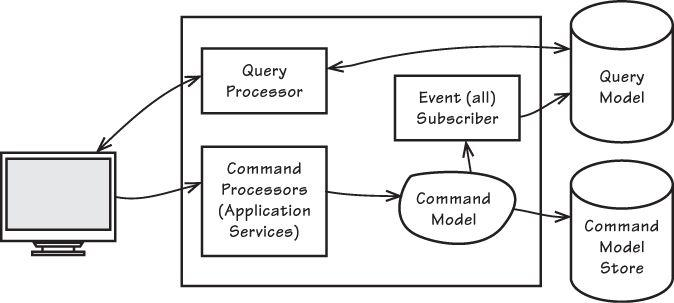
\includegraphics[width=0.9\textwidth]{img/cqrs-diagram.png}
  \end{center}
\end{frame}

\begin{frame}[fragile]{CQRS Java — Command Side}
\begin{lstlisting}[language=Java]
public record CreateUserCommand(String id, String name) {}

public class UserCommandHandler {
    private final UserRepository repo;
    public UserCommandHandler(UserRepository repo) { this.repo = repo; }
    public void handle(CreateUserCommand cmd) {
        repo.save(new User(cmd.id(), cmd.name()));
    }
}
\end{lstlisting}
\end{frame}

\begin{frame}[fragile]{CQRS Java — Query Side}
\begin{lstlisting}[language=Java]
public class UserProjection {
    @EventListener
    public void on(UserCreated e) {
        // 更新 Read Model (denormalized DB)
    }
}

public class UserQueryService {
    private final UserReadRepo repo;
    public UserQueryService(UserReadRepo r) { this.repo = r; }
    public UserDTO fetch(String id) { return repo.find(id); }
}
\end{lstlisting}
\end{frame}


% ================== Section: Event-Driven =====================
% ================== Section: Event-Driven =====================
\section{Event-Driven Architecture}
\begin{frame}{事件驅動架構}
    \begin{itemize}
        \item 服務間透過事件進行非同步通訊
        \item 鬆耦合、高擴展性、最終一致性
        \item 可結合事件溯源(Event Sourcing)模式
    \end{itemize}
    \begin{center}
        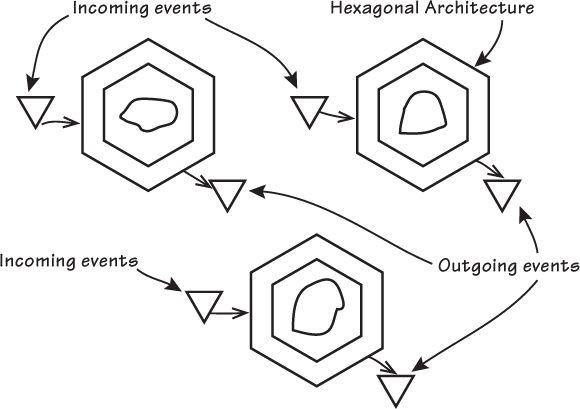
\includegraphics[width=0.7\textwidth]{img/event-driven-hex.png}
    \end{center}
\end{frame}

\begin{frame}[fragile]{Saga 編排範例}
\begin{lstlisting}[language=Java]
class ShippingSaga {
    @SagaEventHandler
    void on(OrderCreated e) {
        send(new ReserveInventory(e.id()));
    }
    @SagaEventHandler
    void on(InventoryReserved e) {
        send(new ArrangeShipment(e.orderId()));
    }
    @SagaEventHandler
    void on(ShipmentArranged e) {
        send(new MarkOrderShipped(e.orderId()));
        end();
    }
}
\end{lstlisting}
\end{frame}

\begin{frame}{事件溯源模式}
  \begin{itemize}
    \item 將 Aggregate 的每次狀態變更以事件持久化 (Append-Only)
    \item 可重播事件重建任何時間點狀態,支援審計與時間旅行
    \item 常與 CQRS / Saga 搭配使用
  \end{itemize}
  \begin{center}
    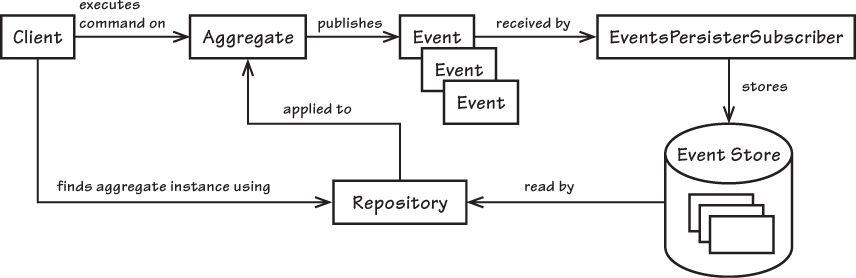
\includegraphics[width=0.7\textwidth]{img/event-sourcing-pipeline.png}
  \end{center}
\end{frame}

\begin{frame}[fragile]{Event Sourcing Java 範例}
\begin{lstlisting}[language=Java]
public interface DomainEvent { Instant occurredAt(); }

public record OrderCreated(String id, Instant occurredAt) implements DomainEvent {}

public class OrderAggregate {
    private String id;
    private OrderStatus status;

    public static OrderAggregate reconstitute(List<DomainEvent> history) {
        OrderAggregate agg = new OrderAggregate();
        history.forEach(agg::apply);
        return agg;
    }
    private void apply(DomainEvent e) {
        if (e instanceof OrderCreated oc) {
            this.id = oc.id();
            this.status = OrderStatus.CREATED;
        }
    }
}
\end{lstlisting}
\end{frame}

% ================== Section: Data Fabric =====================
\section{Data Fabric}
\begin{frame}{Data Fabric 架構要點}
    \begin{itemize}
        \item 統一資料平面:整合 OLTP / OLAP / Streams / Cache
        \item Smart Cache、Federated Query、Consistency Policy、Observability
        \item 與 DDD 聚合分片結合,確保資料局部性與效能
    \end{itemize}
\end{frame}

\begin{frame}[fragile]{Hazelcast 快取範例}
    \begin{lstlisting}[language=Java]
Config cfg = new Config();
HazelcastInstance hz = Hazelcast.newHazelcastInstance(cfg);
IMap<String, OrderSummary> orders = hz.getMap("orders");

OrderSummary summary = new OrderSummary("ID-123", 1023, Instant.now());
orders.set(summary.id(), summary, 30, TimeUnit.MINUTES);

Collection<OrderSummary> highValue = orders.values(
    Predicates.greaterThan("total", 1000));
\end{lstlisting}
\end{frame}

\begin{frame}[fragile]{Apache Ignite 分散運算範例}
    \begin{lstlisting}[language=Java]
Ignition.start();
Ignite ignite = Ignition.ignite();
IgniteCache<Integer, Tick> cache = ignite.getOrCreateCache("ticks");

IgniteCallable<Double> task = () -> {
    List<List<?>> rows = cache.query(
      new SqlFieldsQuery("SELECT price FROM Tick WHERE pid = ?")
        .setArgs(portfolioId)).getAll();
    List<Double> prices = rows.stream()
        .map(r -> (Double) r.get(0))
        .sorted()
        .collect(Collectors.toList());
    return prices.get((int)(prices.size() * 0.05)); // Value-at-Risk
};

Double var = ignite.compute().call(task);
\end{lstlisting}
\end{frame}

\begin{frame}{Data Fabric 風險與治理建議}
    \begin{itemize}
        \item \textbf{記憶體壓力}:熱資料量估錯 → OOM,建議 TTL + LRU Eviction
        \item \textbf{Schema 演進}:需有 Registry + 相容性驗證
        \item \textbf{Split-Brain}:多區部署需啟用 CP 模式或資料同步機制
        \item \textbf{安全}:敏感資料須加密(靜態/傳輸/使用中)與審計紀錄
    \end{itemize}
\end{frame}

% ================== 結語 =====================
\section{結語}
\begin{frame}{結語:架構即演進}
    \begin{itemize}
        \item 沒有銀彈架構,DDD 幫助你因應變化、協作清晰
        \item 每種架構風格皆服務於 Domain 模型的演進
        \item 避免技術導向的「錯配式設計」;堅持語言一致性與 Context 純度
        \item 架構設計的重點不是「選哪一種」,而是「如何隨著需求演進」
    \end{itemize}
\end{frame}

\begin{frame}[plain,noframenumbering]
    \centering
    \Huge \textbf{謝謝收看!} \\
    \vspace{1cm}
    \normalsize Slides by
\end{frame}

\end{document}
